\subsection{Experimental Setup}
\label{sec:setup}

\subsubsection{System used}

We employ a server equipped with two Intel Xeon Gold 6226R processors, each featuring $16$ cores running at a clock speed of $2.90$ GHz. Each core is equipped with a $1$ MB L1 cache, a $16$ MB L2 cache, and a $22$ MB shared L3 cache. The system is configured with $376$ GB RAM and set up with CentOS Stream 8.


\subsubsection{Configuration}

We use 32-bit integers for vertex ids and 32-bit float for edge weights but use 64-bit floats for computations and hashtable values. We utilize $64$ threads to match the number of cores available on the system (unless specified otherwise). For compilation, we use GCC 8.5 and OpenMP 4.5.


\subsubsection{Dataset}

The graphs used in our experiments are given in Table \ref{tab:dataset}. These are sourced from the SuiteSparse Matrix Collection \cite{suite19}. In the graphs, number of vertices vary from $3.07$ to $214$ million, and number of edges vary from $25.4$ million to $3.80$ billion. We ensure edges to be undirected and weighted with a default of $1$.

\begin{table}[hbtp]
  \centering
  \caption{List of $13$ graphs obtained SuiteSparse Matrix Collection \cite{suite19} (directed graphs are marked with $*$). Here, $|V|$ is the number of vertices, $|E|$ is the number of edges (after adding reverse edges), $D_{avg}$ is the average degree, and $|\Gamma|$ is the number of communities obtained using Louvain algorithm.\ignore{In the table, B refers to a billion, M refers to a million and K refers a thousand.}}
  \label{tab:dataset}
  \begin{tabular}{|c||c|c|c|c|}
    \toprule
    \textbf{Graph} &
    \textbf{\textbf{$|V|$}} &
    \textbf{\textbf{$|E|$}} &
    \textbf{\textbf{$D_{avg}$}} &
    \textbf{\textbf{$|\Gamma|$}} \\
    % \textbf{$1 - \Gamma_G$} \\
    \midrule
    \multicolumn{5}{|c|}{\textbf{Web Graphs (LAW)}} \\ \hline
    indochina-2004$^*$ & 7.41M & 341M & 41.0 & 4.24K \\ \hline  % & \num{4.7e-4} & 2.9 GB
    uk-2002$^*$ & 18.5M & 567M & 16.1 & 42.8K \\ \hline  % & \num{9.6e-5} & 16 GB
    arabic-2005$^*$ & 22.7M & 1.21B & 28.2 & 3.66K \\ \hline  % & \num{5.5e-4} & 11 GB
    uk-2005$^*$ & 39.5M & 1.73B & 23.7 & 20.8K \\ \hline  % & \num{9.6e-5} & 16 GB
    webbase-2001$^*$ & 118M & 1.89B & 8.6 & 2.76M \\ \hline  % & \num{7.3e-7} & 18 GB
    it-2004$^*$ & 41.3M & 2.19B & 27.9 & 5.28K \\ \hline  % & \num{3.8e-4} & 19 GB
    sk-2005$^*$ & 50.6M & 3.80B & 38.5 & 3.47K \\ \hline  % & \num{5.8e-4} & 33 GB
    \multicolumn{5}{|c|}{\textbf{Social Networks (SNAP)}} \\ \hline
    com-LiveJournal & 4.00M & 69.4M & 17.4 & 2.54K \\ \hline  % & \num{7.9e-4} & 480 MB
    com-Orkut & 3.07M & 234M & 76.2 & 29 \\ \hline  % & \num{6.7e-2} & 1.7 GB
    \multicolumn{5}{|c|}{\textbf{Road Networks (DIMACS10)}} \\ \hline
    asia\_osm & 12.0M & 25.4M & 2.1 & 2.38K \\ \hline  % & \num{8.4e-4} & 200 MB
    europe\_osm & 50.9M & 108M & 2.1 & 3.05K \\ \hline  % & \num{6.6e-4} & 910 MB
    \multicolumn{5}{|c|}{\textbf{Protein k-mer Graphs (GenBank)}} \\ \hline
    kmer\_A2a & 171M & 361M & 2.1 & 21.2K \\ \hline  % & \num{9.4e-5} & 3.2 GB
    kmer\_V1r & 214M & 465M & 2.2 & 6.17K \\ \hline  % & \num{3.2e-4} & 4.2 GB
  \bottomrule
  \end{tabular}
\end{table}
% We convert directed graphs (marked with $*$) to undirected by duplicating edges in the reverse direction, and set the weight of each edge to $1$. and $F_{size}$ is size of the \textit{MatrixMarket} file

\begin{figure*}[hbtp]
  \centering
  \subfigure[Runtime in seconds (logarithmic scale) with \textit{Original Leiden}, \textit{igraph Leiden}, \textit{NetworKit Leiden}, and \textit{GVE-Leiden}]{
    \label{fig:leiden-compare--runtime}
    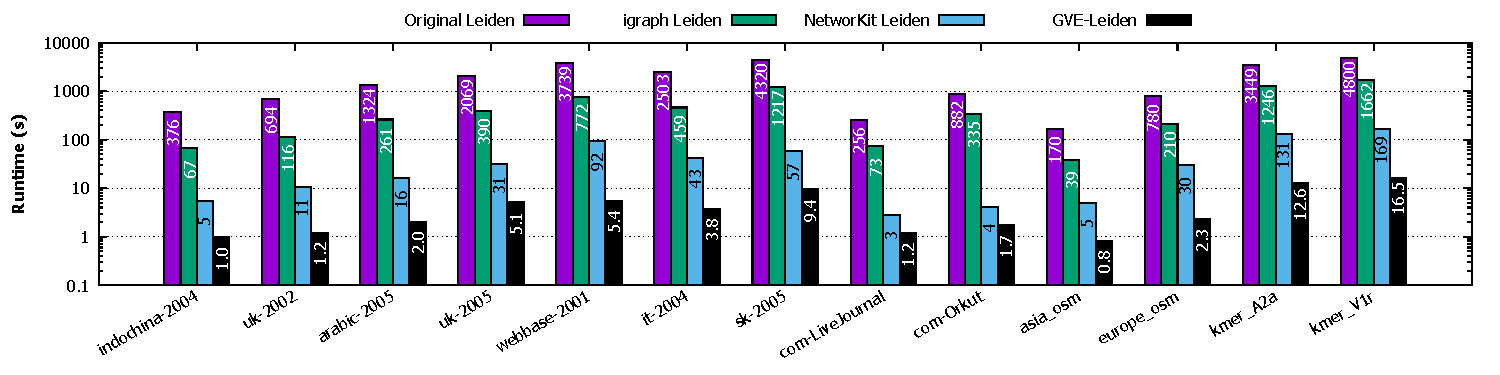
\includegraphics[width=0.98\linewidth]{out/leiden-runtime.pdf}
  } \\[-0ex]
  \subfigure[Speedup of \textit{GVE-Leiden} (logarithmic scale) with respect to \textit{Original Leiden}, \textit{igraph Leiden}, \textit{NetworKit Leiden}.]{
    \label{fig:leiden-compare--speedup}
    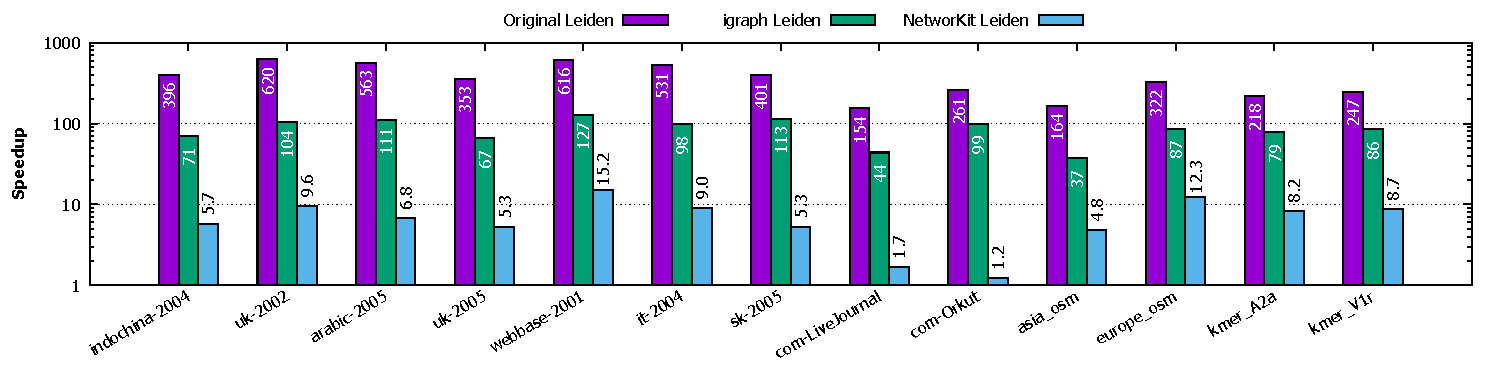
\includegraphics[width=0.98\linewidth]{out/leiden-speedup.pdf}
  } \\[-0ex]
  \subfigure[Modularity of communities obtained with \textit{Original Leiden}, \textit{igraph Leiden}, \textit{NetworKit Leiden}, and \textit{GVE-Leiden}.]{
    \label{fig:leiden-compare--modularity}
    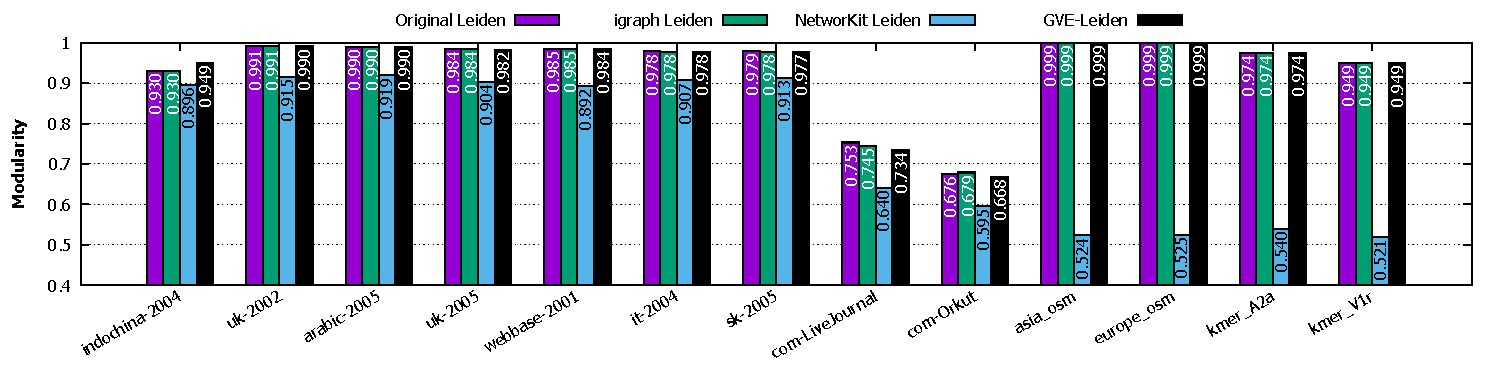
\includegraphics[width=0.98\linewidth]{out/leiden-modularity.pdf}
  } \\[-0ex]
  \subfigure[Fraction of disconnected communities (logarithmic scale) with \textit{Original Leiden}, \textit{igraph Leiden}, \textit{NetworKit Leiden}, and \textit{GVE-Leiden}.]{
    \label{fig:leiden-compare--disconnected}
    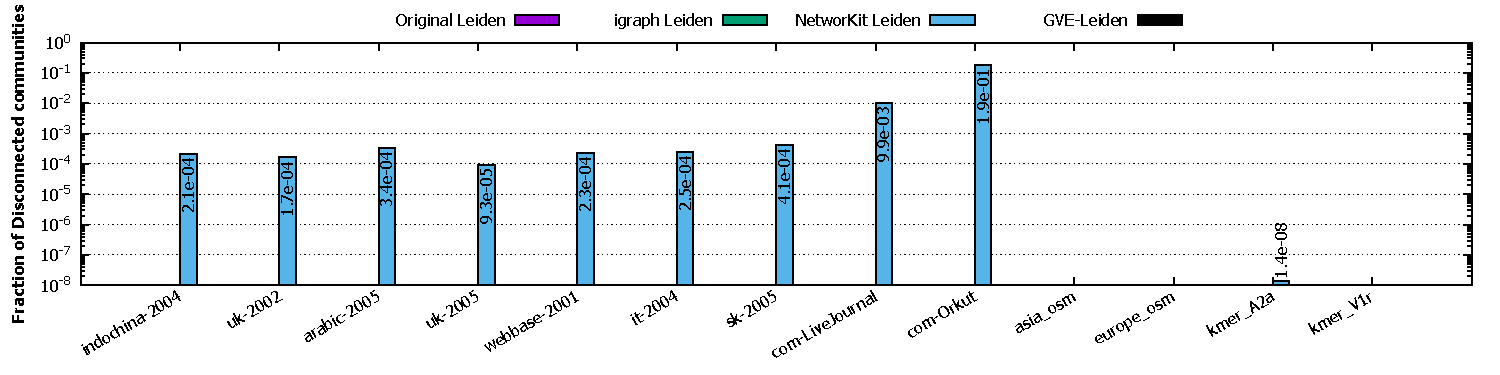
\includegraphics[width=0.98\linewidth]{out/leiden-disconnected.pdf}
  } \\[-2ex]
  \caption{Runtime in seconds (log-scale), speedup (log-scale), modularity, and fraction of disconnected communities (log-scale) with \textit{Original Leiden}, \textit{igraph Leiden}, \textit{NetworKit Leiden}, and \textit{GVE-Leiden} for each graph in the dataset.}
  \label{fig:leiden-compare}
\end{figure*}

\begin{figure*}[hbtp]
  \centering
  \subfigure[Runtime in seconds (logarithmic scale) with \textit{GVE-Louvain} and \textit{GVE-Leiden}]{
    \label{fig:gve-compare--runtime}
    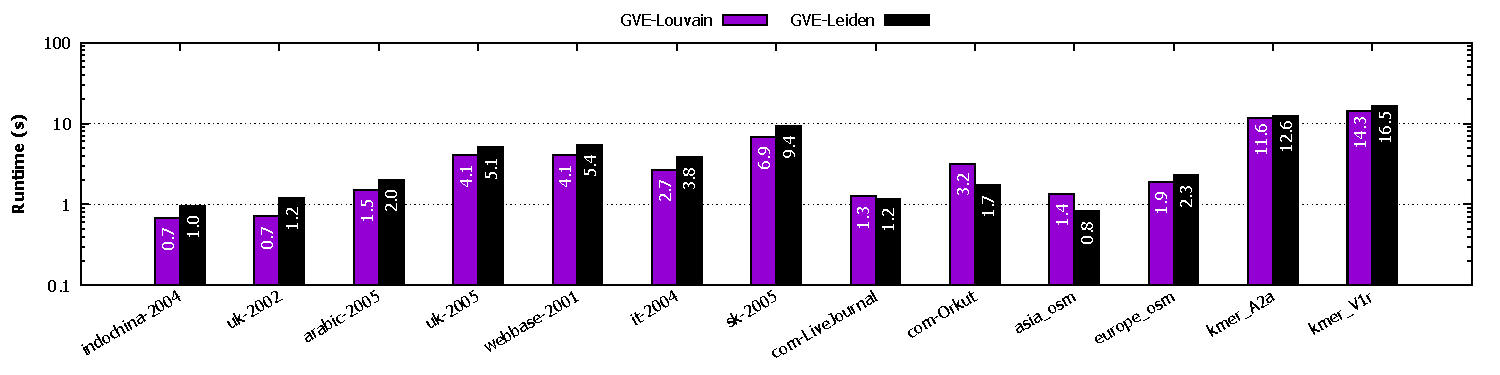
\includegraphics[width=0.98\linewidth]{out/gve-runtime.pdf}
  } \\[-0ex]
  \subfigure[Speedup of \textit{GVE-Leiden} with respect to \textit{GVE-Louvain}. \textit{GVE-Leiden} is generally slower (speedup < $1$) because of additional refinement phase.]{
    \label{fig:gve-compare--speedup}
    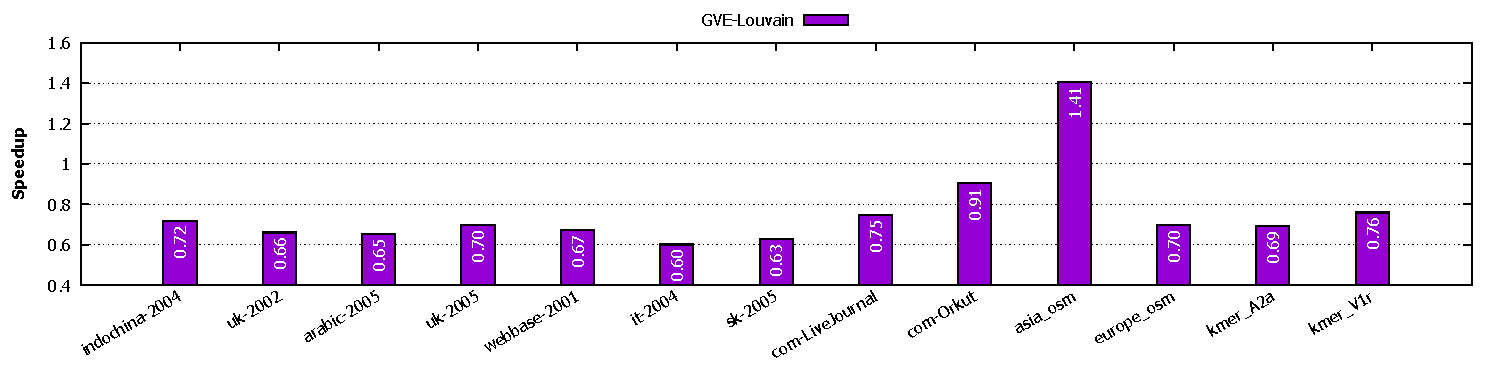
\includegraphics[width=0.98\linewidth]{out/gve-speedup.pdf}
  } \\[-0ex]
  \subfigure[Modularity of communities obtained with \textit{GVE-Louvain} and \textit{GVE-Leiden}.]{
    \label{fig:gve-compare--modularity}
    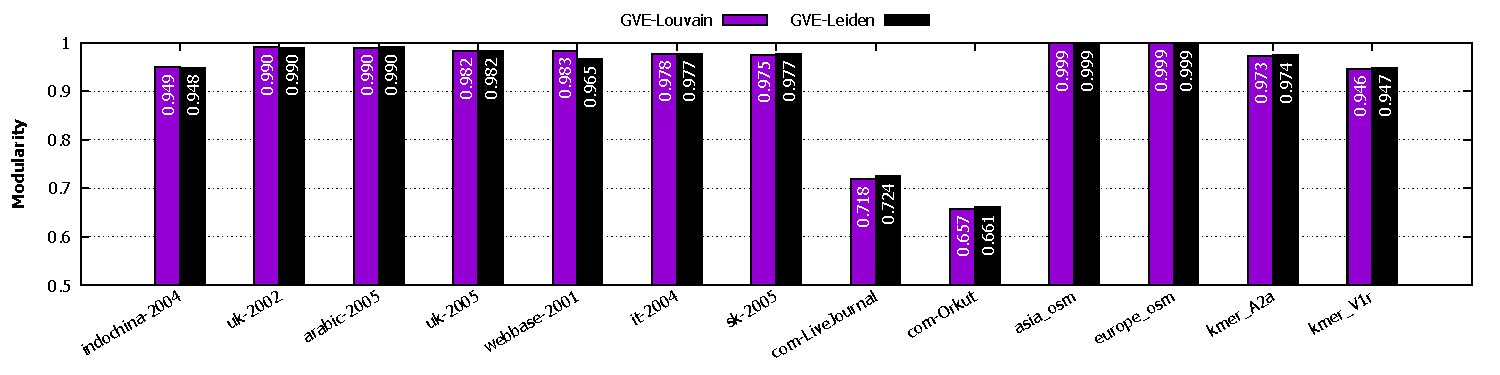
\includegraphics[width=0.98\linewidth]{out/gve-modularity.pdf}
  } \\[-0ex]
  \subfigure[Fraction of disconnected communities (logarithmic scale) with \textit{GVE-Louvain} and \textit{GVE-Leiden}.]{
    \label{fig:gve-compare--disconnected}
    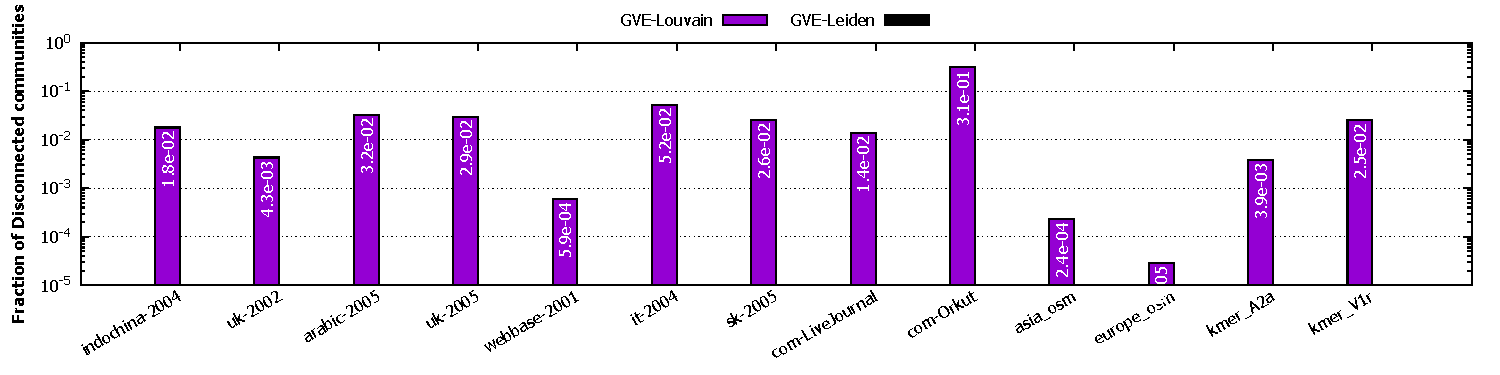
\includegraphics[width=0.98\linewidth]{out/gve-disconnected.pdf}
  } \\[-2ex]
  \caption{Runtime in seconds (log-scale), speedup, modularity, and fraction of disconnected communities (log-scale) with \textit{GVE-Louvain} and \textit{GVE-Leiden} for each graph in the dataset.}
  \label{fig:gve-compare}
\end{figure*}





\subsection{Comparing Performance of GVE-Leiden}

We now compare the performance of GVE-Leiden with Vite (Louvain), Grappolo (Louvain), and NetworKit Louvain. For Vite, we convert the graph datasets to Vite's binary graph format, run it on a single node\ignore{(Vite supports distributed community detection)} with threshold cycling/scaling optimization, and measure the reported average total time. For Grappolo, we measure the run it on the same system, and measure the reported total time. For NetworKit, we use a Python script to invoke \texttt{PLM} (Parallel Louvain Method), and measure the total time reported with \texttt{getTiming()}. For each graph, we measure the runtime of each implementation five times, for averaging. We also record the modularity of communities obtained, as reported by each implementation.

Figure \ref{fig:leiden-compare--runtime} shows the runtimes of Vite (Louvain), Grappolo (Louvain), NetworKit Louvain, and GVE-Leiden on each graph in the dataset. Figure \ref{fig:leiden-compare--speedup} shows the speedup of GVE-Leiden with respect to each implementation mentioned above. GVE-Leiden is on average $50\times$, $22\times$, and $20\times$ faster than Vite, Grappolo, and NetworKit respectively. On the \textit{sk-2005} graph, GVE-Leiden finds communities in $6.8$ seconds, and thus achieve a processing rate of $560$ million edges/s. Figure \ref{fig:leiden-compare--modularity} shows the modularity of communities obtained with each implementation. GVE-Leiden on average obtains $3.1\%$ higher modularity than Vite (especially on web graphs), and $0.6\%$ lower modularity than Grappolo and NetworKit (especially on social networks with poor clustering).

\begin{figure*}[hbtp]
  \centering
  \subfigure[Phase split]{
    \label{fig:leiden-splits--phase}
    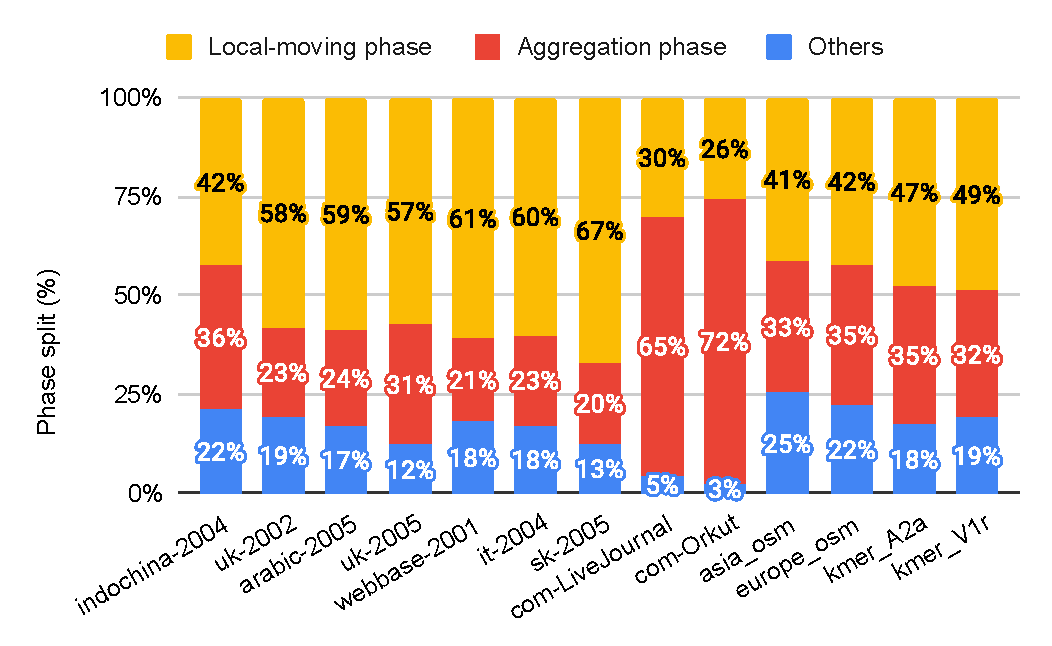
\includegraphics[width=0.48\linewidth]{out/leiden-phases.pdf}
  }
  \subfigure[Pass split]{
    \label{fig:leiden-splits--pass}
    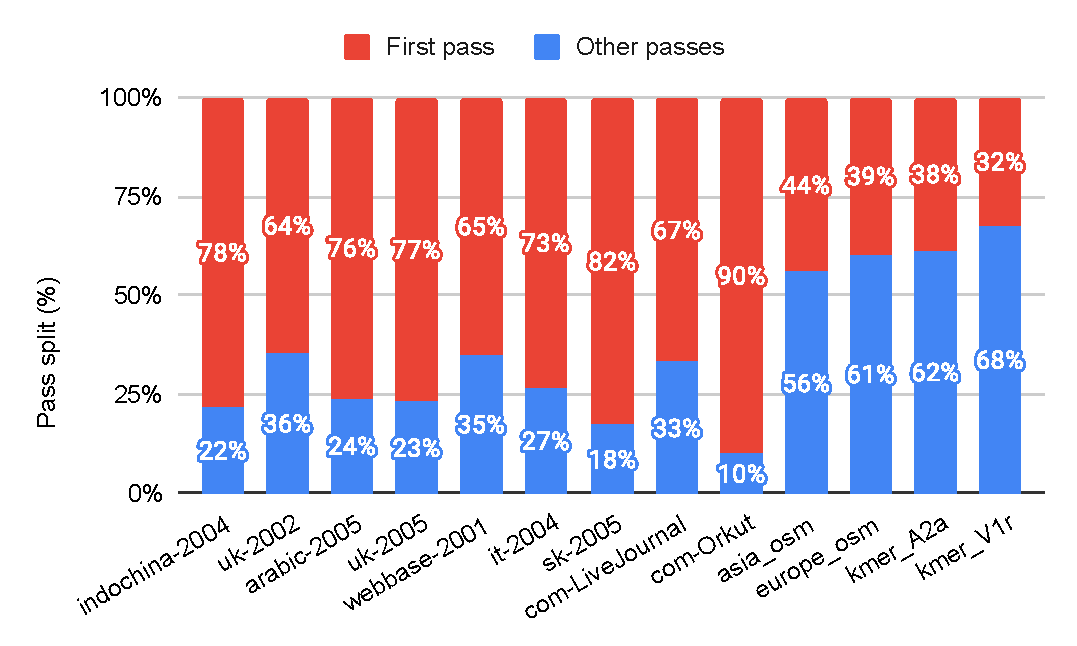
\includegraphics[width=0.48\linewidth]{out/leiden-passes.pdf}
  } \\[-2ex]
  \caption{Phase split of \textit{GVE-Leiden} shown on the left, and pass split shown on the right for each graph in the dataset.}
  \label{fig:leiden-splits}
\end{figure*}

\begin{figure}[hbtp]
  \centering
  \subfigure{
    \label{fig:leiden-hardness--all}
    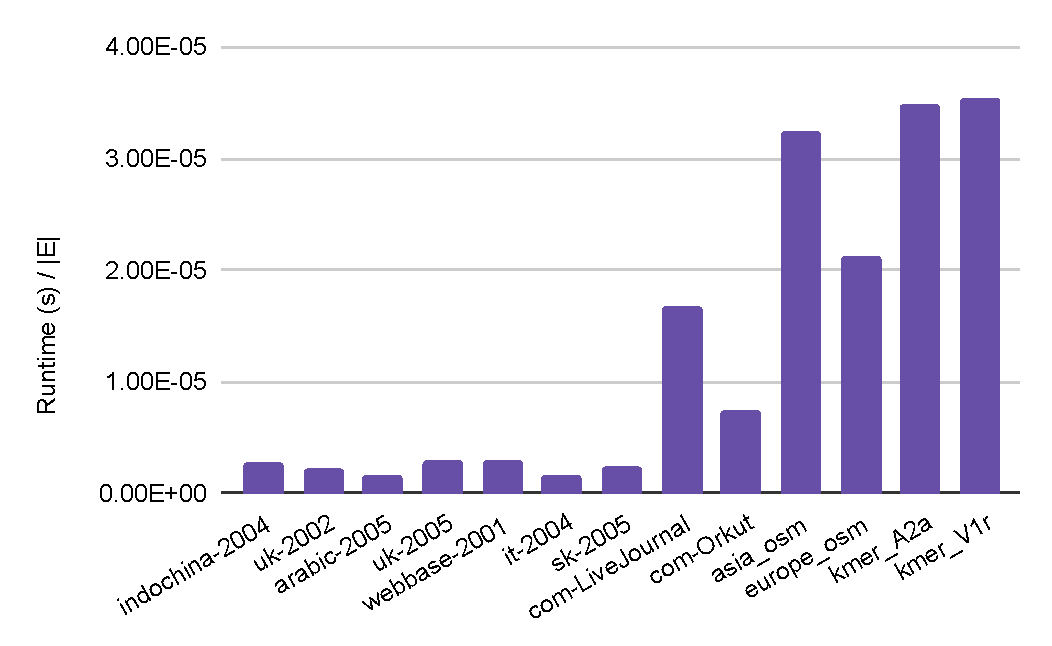
\includegraphics[width=0.98\linewidth]{out/leiden-hardness.pdf}
  } \\[-2ex]
  \caption{Runtime $/ |E|$ factor with \textit{GVE-Leiden} for each graph in the dataset.}
  \label{fig:leiden-hardness}
\end{figure}

\begin{figure}[hbtp]
  \centering
  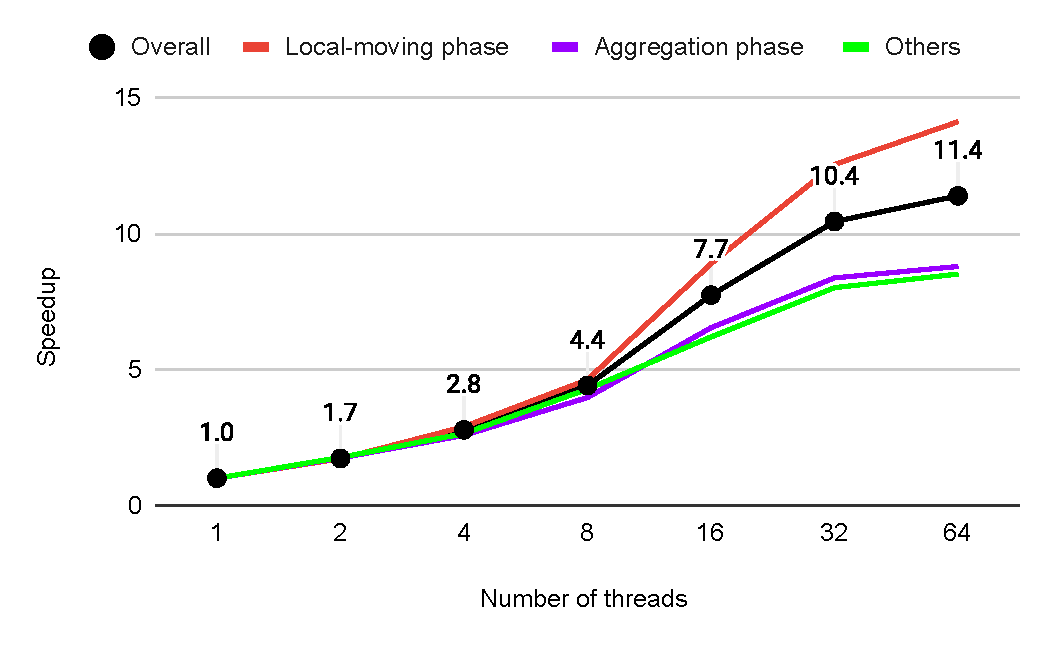
\includegraphics[width=0.98\linewidth]{out/leiden-ss.pdf} \\[-2ex]
  \caption{Overall speedup of \textit{GVE-Leiden}, and its various phases (local-moving, refinement, aggregation, others), with increasing number of threads (in multiples of 2).}
  \label{fig:leiden-ss}
\end{figure}





\subsection{Analyzing Performance of GVE-Leiden}

%% Disconnected communities with Leiden algorithm
From the initial results it looks like Leiden algorithm is much less likely than Louvain to return disconnected communities. However, the modularity obtained is generally (interestingly) generally lower than PageRank. Also the randomized version of refinement phase of Leiden (using xorshift32 random engine) somehow seems to obtain lower modularity than greedy version of refinement phase.

The phase-wise and pass-wise split of GVE-Leiden is shown in Figures \ref{fig:leiden-splits--phase} and \ref{fig:leiden-splits--pass} respectively. Figure \ref{fig:leiden-splits--phase} indicates that GVE-Leiden spends most of the runtime in the local-moving phase on \textit{web graphs}, \textit{road networks}, and \textit{protein k-mer graphs}, while it devotes majority of the runtime in the aggregation phase on \textit{social networks}. The pass-wise split (Figure \ref{fig:leiden-splits--pass}) indicates that the first pass dominates runtime on high-degree graphs (\textit{web graphs} and \textit{social networks}), while subsequent passes prevail in execution time on low-degree graphs (\textit{road networks} and \textit{protein k-mer graphs}).

On average, $49\%$ of GVE-Leiden's runtime is spent in the local-moving phase, $35\%$ is spent in the aggregation phase, and $16\%$ is spent in other steps (initialization, renumbering communities, looking up dendrogram, and resetting communities) of the algorithm. Further, $67\%$ of the runtime is spent in the first pass of the algorithm, which is the most expensive pass due to the size of the original graph (later passes work on super-vertex graphs) \cite{com-wickramaarachchi14}.

We also observe that graphs with lower average degree (\textit{road networks} and \textit{protein k-mer graphs}) and graphs with poor community structure (such as \verb|com-LiveJournal| and \verb|com-Orkut|) have a larger $\text{runtime}/|E|$ factor, as shown in Figure \ref{fig:leiden-hardness}.


%% Additional analysis for Leiden algorithm
In this section, we observe the performance of our optimized parallel \textit{Leiden} (\textit{greedy variant}) with respect to \textit{Louvain} (which is optimized and parallelized in a manner similar to \textit{Leiden}). For each graphs in the dataset, we run each algorithm 5 times to minimize measurement noise, and report the average results in Figures \ref{fig:leiden-disconnected}, \ref{fig:leiden-modularity}, and \ref{fig:leiden-time}.

Figure \ref{fig:leiden-disconnected} shows the percentage of disconnected communities obtained with both algorithms for each graph in the dataset. \textit{Leiden} obtains drastically reduced number of disconnected communities compared to \textit{Louvain} (except on road networks), achieving an average of $20\times$ reduction in disconnected communities. Meanwhile, Figure \ref{fig:leiden-modularity} shows the modularity of both algorithms on the same dataset. We observe that \textit{Leiden}, on average, obtains communities of slightly higher modularity than \textit{Louvain}. Lastly, Figure \ref{fig:leiden-time} shows the runtime of both algorithms across the dataset. \textit{Leiden} is on average $26\%$ slower than Louvain. Nonetheless, this increase in computation time is a minor trade-off for obtaining predominantly well-connected high-quality communities.




\subsection{Strong Scaling of GVE-Leiden}

Finally, we measure the strong scaling performance of GVE-Leiden. To this end, we adjust the number of threads from $1$ to $64$ in multiples of $2$ for each input graph, and measure the overall time taken for finding communities with GVE-Leiden, as well as its phase splits (local-moving, aggregation, others), five times for averaging. The results are shown in Figure \ref{fig:leiden-ss}. With 32 threads, GVE-Leiden obtains an average speedup of $10.4\times$ compared to running with a single thread, i.e., its performance increases by $1.6\times$ for every doubling of threads. Scaling is limited due to the various sequential steps/phases in the algorithm. At 64 threads, GVE-Leiden is impacted by NUMA effects, and offers speedup of only $11.4\times$.
